\documentclass[a4paper,12pt]{article}
\usepackage[margin=1in]{geometry}

\usepackage[T2A]{fontenc}			% кодировка
\usepackage[utf8]{inputenc}			% кодировка исходного текста
\usepackage[english,russian]{babel}	% локализация и переносы
\usepackage{graphicx}                % Математика
\usepackage{amsmath,amsfonts,amssymb,amsthm,mathtools} 
\usepackage{mathtext}
\usepackage[T2A]{fontenc}
\usepackage[utf8]{inputenc}

\usepackage{wasysym}

%Заговолок
\author{ \Бичина Марина 
группа Б04-005 1 курса ФЭФМ}
\title{}
\date{}


\begin{document} % начало документа

\begin{center}
\begin{Large}
{Бичина Марина Б04-005, Лабораторная работа №. 4.1.1 <<Изучение центрированных оптических систем>>}
\end{Large}
\end{center}
\paragraph{Цель работы:} 
\begin{enumerate}
\itemsep0em
\item изучить методы определения фокусных расстояний линз и сложных оптических систем
\item определить характеристики оптической системы, составленной из тонких линз

\end{enumerate}
\paragraph{Оборудование:}
\begin{enumerate}
\itemsep0em
\item оптическая скамья с набором рейтеров
\item положительные и отрицательные линзы
\item экран
\item осветитель
\item зрительная труба
\item светофильтры
\item кольцевые диафрагмы
\item линейка
\end{enumerate}

\paragraph{Теоретическая справка:}
\begin{enumerate}
\item Определение фокусного расстояния тонкой собирающей линзы методом Аббе
\begin{figure}[h!]
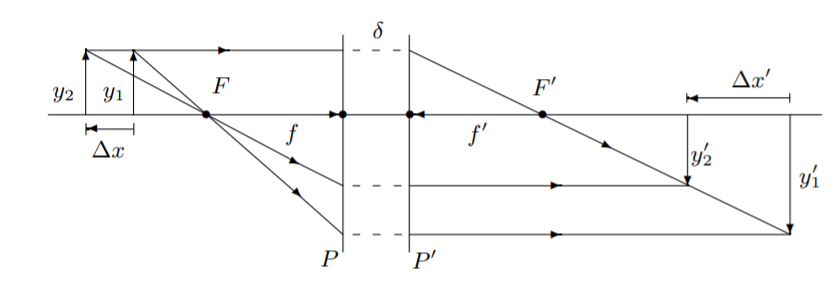
\includegraphics[scale=1]{abbe.png} 
\caption{Измерение фокусного расстояния оптической системы по методу Аббе}
\end{figure}
Измерение фокусного расстояния по методу Аббе основано на определении поперечного увеличения для нескольких различных положений предмета. Рассчеты производятся следующим образом:
\begin{equation}
f = \frac{\Delta x}{\Delta(y/y')} = -\frac{\Delta x'}{\Delta (y'/y)}
\end{equation}
где $\Delta(y'/y)=y_2/y'_2-y_1/y'_1$ - приращение поперечного увеличения, а $\Delta(y/y')$ - величина, обратная поперечному увеличению
\item Определение фокусного расстояния собирающих линз и сложных оптических систем методом Бесселя

Метод основан на том, что при заданном расстоянии
L между предметом и экраном уравнение 
\begin{equation}
\frac{-1}{s}+\frac{1}{s'} = \frac{1}{f}
\end{equation}
 представляет собой
квадратное уравнение относительно расстояния s от главной плоскости пространства предметов до предмета
\begin{equation}
\frac{-1}{s}+\frac{1}{L-\delta +s} = \frac{1}{f}
\end{equation}
\begin{figure}[h!]
\centering
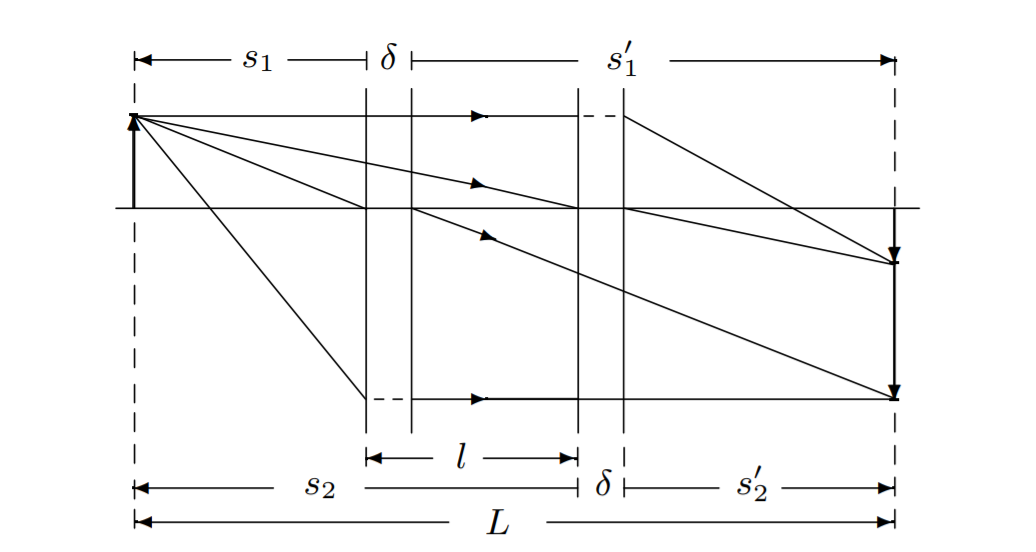
\includegraphics[scale=0.75]{besel.png} 
\caption{Измерение фокусного расстояние методом Бесселя}
\end{figure}

В ходе преобразований формула фокуса может быть представлена в виде 
\begin{equation}
f =\frac{L^2-l^2}{4L}
\end{equation}
где L - расстояние между предметом и экраном, l - расстояние между двумя положениями системы, при которых видны четкие изображения
\end{enumerate}

\paragraph{Ход работы:}
\begin{enumerate}
\itemsep0em
\item Определение фокусных расстояний тонких линз при помощи экрана
\begin{enumerate}
\itemsep0em
\item Метод Аббе  (собирающая линза 1)
\begin{figure}[h!]
\centering
\begin{tabular}{|c|c|c|c|}
\hline 
$x_1$, см & $x_1'$, см & $y_1$, см & $y_1'$, см \\ 
\hline 
17.5 & 31 & 2 & 5 \\ 
\hline 
$x_2$, см & $x_2'$, см & $y_2$, см & $y_2'$, см \\ 
\hline 
15 & 51.5 & 2 & 8.5 \\ 
\hline 
\end{tabular}
\caption{Данные, полученные методом Аббе для 1 линзы} 
\end{figure}
По формуле 1:\\

\[f_1 = \frac{2.5}{85/14} = 15.18\;\;\text{см}\]
или
\[f_1 = \frac{20.5}{7/4} = 11.71\;\;\text{см}\]
Погрешность:\\
\[\varepsilon_f = \sqrt{(\sqrt{2}\cdot\sigma x/(x_2-x_1))^2+ (\frac{\dfrac{y\sigma x}{y_1^2}}{\dfrac{y_2}{y_2'} - \dfrac{y_1}{y_1'}})^2}\approx 0.75\]
\[\sigma_f = 1.5\cdot 11.71 = 8.8\;\;\text{см}\]
Погрешность получилась огромная, поскольку у нас оказалось 2 совершенно разных значения для одной и той же линзы\\ 
Пока мы не можем точно сказать, чему равняется значение для линзы, перейдем к следующему способу для измерения фокусного расстояния\\

\item Метод Бесселя
\begin{figure}[h!]
\centering\begin{tabular}{|c|c|c|c|c|c|}
\hline 
$s_1$, см & $s_1'$, см & $s_2$, см & $s_2'$, см & L, см & l, см \\ 
\hline 
15 & 55.5 & 57.5 & 13.5 & 71 & 41 \\ 
\hline 
\end{tabular} 
\caption{Усредненные данные, полученные методом Бесселя для 1 линзы}
\end{figure}
\[f_1 = \dfrac{71^2-42^2}{4\cdot 71} = 11.53\;\;\text{см}\]
\begin{figure}[h!]
\centering
\begin{tabular}{|c|c|c|}
\hline 
$a_0$, см & $a'$, см & l, см \\ 
\hline 
14.5 & 13.5 & 8 \\ 
\hline
\end{tabular} 
\caption{Данные, полученные методом Бесселя для рассеивающей линзы}
\end{figure}
\[\frac{1}{f}=\frac{1}{a'}-\frac{1}{a_0-l} = \frac{(a_0-l)a'}{a_0-l-a'} = \frac{6.5 \cdot 13.5}{6.5 - 13.5} = -12.54\;\;\text{см}\]
\end{enumerate}
Погрешность:\\
\[\varepsilon_f=\sqrt{2}\cdot\sqrt{(\frac{\sqrt{L^2 + l^2}}{L^2 - l^2})^2+(\frac{L^2\frac{(2\sigma x)}{L}}{L^2})^2} = 0.05\;\;\text{см}\]
\[\sigma_f= 0.05\cdot 11.53 = 0.6\;\;\text{см}\]
$f = 11.53 \pm 0.6$ см \\
$f = -12.54 \pm 0.6$ см \\
\item Определение фокусных расстояний тонких линз с помощью зрительной трубы
\begin{figure}[h!]
\centering
\begin{tabular}{|c|c|c|}
\hline 
 & Линза 1 & Линза 2 \\ 
\hline 
1 сторона & 12 & 14.5 \\ 
\hline 
2 сторона & 11.5 & 14.5 \\ 
\hline 
\end{tabular} 
\end{figure}
Рассеивающая линза:\\
$a_0 = 28$ см\\
$l = 15.5$ см\\
$f = a_0-l = 12.5$ см\\ 
$f = 12.5 \pm 0.6$ см\\
Инструментальную погрешность считаем равной 0.5 см из-за не совсем точных измерений (неточно определены центры линз, идет смещение из-за рейтеров)

Итого получаем:
\begin{figure}[h!]
\centering
\begin{tabular}{|c|c|c|}
\hline 
Линза & f, см & D, cм$^{-1}$ \\ 
\hline 
1 (собирающая) & 11.53 & 0.087 \\ 
\hline 
2 (собирающая) & 14.5 & 0.069 \\ 
\hline 
3 (рассеивающая) & -12.54 & 0.080 \\ 
\hline 
\end{tabular} 
\end{figure}

\item Определение фокусного расстояния и положения главных и
фокальных плоскостей сложной оптической системы
\begin{figure}[h!]
\centering
\begin{tabular}{|c|c|c|c|c|c|c|}
\hline 
y, см & $y_1'$, см & $y_2'$, см & $x_1$, см & $x_1'$, см & $x_2$, см & $x_2'$, см \\ 
\hline 
2 & 8.5 & 3 & 12.5 & 40 & 9.5 & 33 \\ 
\hline 
\end{tabular} 
\end{figure}

\begin{enumerate}
\itemsep0em
\item Найдем главные фокусные расстояния системы:\\
Более реалистичное значение для фокусного расстояния
$f_{1\Sigma} \approx 9\;\;\text{см}$
\end{enumerate}
\item Нахождение главных фокусов системы с помощью зрительной трубы:
\[F_{1\Sigma}=6.5 \pm 0.5\;\;\text{см}\]
\[F_{2\Sigma} = 4.6\pm 0.5\;\;\text{см}\;\;\;\;\text{(когда линзы поменяли местами)}\]
\item Определим вычислительно значения для $H_1, H_2, F_1, F_2, f_2$
\[H_1 = \frac{f_1\cdot l_{12}}{l_{12} - f_1 - f_2} = 3.1\;\;\text{см}\]
\[H_2 = \frac{f_2\cdot l_{12}}{l_{12} - f_1 - f_2} = 3.9\;\;\text{см}\]
\[F_1 = f_1(1 + \frac{f_1}{l_{12} - f_1 - f_2}) = 5.0\;\;\text{см}\]
\[F_2 = f_2(1 + \frac{f_2}{l_{12} - f_1 - f_2}) = 4.2\;\;\text{см}\]
\[f_{\Sigma} = \frac{f_1f_2}{l_{12} - f_1-f_2} = 8.1 \;\;\text{см}\]
\item Определим характеристики систем с помощью чертежа:
\[f_{1\Sigma} = 6.7\pm 0.2\;\;\text{см}\]
\[f_{2\Sigma} = 6.6\pm 0.2\;\;\text{см}\]
\[F_{1\Sigma} = 5.0\pm 0.2\;\;\text{см}\]
\[F_{2\Sigma} = 4.4\pm 0.2\;\;\text{см}\]
Видим, что на чертеже значения рассчитаны достаточно точно
\end{enumerate}
\paragraph{Выводы:}
\begin{enumerate}
\item Мы нашли фокусные расстояния для 3-х линз 3 разными способами: Методом Аббе, Бесселя и с помощью зрительной трубы
\[f_1 = 11.5\pm 0.6\;\;\text{см}\]
\[f_2 = 14.5\pm 0.5\;\;\text{см}\]
\[f_2 = 12.5\pm 0.5\;\;\text{см}\]
\item Нашли характеристики сложных систем с помощью зрительной трубы и с помощью чертежа
\[f_{1\Sigma} = 6.7\pm 0.2\;\;\text{см}\]
\[f_{2\Sigma} = 6.6\pm 0.2\;\;\text{см}\]
\[F_{1\Sigma} = 5.0\pm 0.2\;\;\text{см}\]
\[F_{2\Sigma} = 4.4\pm 0.2\;\;\text{см}\]
\end{enumerate}
\end{document}